
%% bare_conf.tex
%% V1.3
%% 2007/01/11
%% by Michael Shell
%% See:
%% http://www.michaelshell.org/
%% for current contact information.
%%
%% This is a skeleton file demonstrating the use of IEEEtran.cls
%% (requires IEEEtran.cls version 1.7 or later) with an IEEE conference paper.
%%
%% Support sites:
%% http://www.michaelshell.org/tex/ieeetran/
%% http://www.ctan.org/tex-archive/macros/latex/contrib/IEEEtran/
%% and
%% http://www.ieee.org/
%%*************************************************************************
%% Legal Notice:
%% This code is offered as-is without any warranty either expressed or
%% implied; without even the implied warranty of MERCHANTABILITY or
%% FITNESS FOR A PARTICULAR PURPOSE! 
%% User assumes all risk.
%% In no event shall IEEE or any contributor to this code be liable for
%% any damages or losses, including, but not limited to, incidental,
%% consequential, or any other damages, resulting from the use or misuse
%% of any information contained here.
%%
%% All comments are the opinions of their respective authors and are not
%% necessarily endorsed by the IEEE.
%%
%% This work is distributed under the LaTeX Project Public License (LPPL)
%% ( http://www.latex-project.org/ ) version 1.3, and may be freely used,
%% distributed and modified. A copy of the LPPL, version 1.3, is included
%% in the base LaTeX documentation of all distributions of LaTeX released
%% 2003/12/01 or later.
%% Retain all contribution notices and credits.
%% ** Modified files should be clearly indicated as such, including  **
%% ** renaming them and changing author support contact information. **
%%
%% File list of work: IEEEtran.cls, IEEEtran_HOWTO.pdf, bare_adv.tex,
%%                    bare_conf.tex, bare_jrnl.tex, bare_jrnl_compsoc.tex
%%*************************************************************************

% *** Authors should verify (and, if needed, correct) their LaTeX system  ***
% *** with the testflow diagnostic prior to trusting their LaTeX platform ***
% *** with production work. IEEE's font choices can trigger bugs that do  ***
% *** not appear when using other class files.                            ***
% The testflow support page is at:
% http://www.michaelshell.org/tex/testflow/



% Note that the a4paper option is mainly intended so that authors in
% countries using A4 can easily print to A4 and see how their papers will
% look in print - the typesetting of the document will not typically be
% affected with changes in paper size (but the bottom and side margins will).
% Use the testflow package mentioned above to verify correct handling of
% both paper sizes by the user's LaTeX system.
%
% Also note that the "draftcls" or "draftclsnofoot", not "draft", option
% should be used if it is desired that the figures are to be displayed in
% draft mode.
%
\documentclass[conference]{IEEEtran}
% Add the compsoc option for Computer Society conferences.
%
% If IEEEtran.cls has not been installed into the LaTeX system files,
% manually specify the path to it like:
% \documentclass[conference]{../sty/IEEEtran}





% Some very useful LaTeX packages include:
% (uncomment the ones you want to load)


% *** MISC UTILITY PACKAGES ***
%
%\usepackage{ifpdf}
% Heiko Oberdiek's ifpdf.sty is very useful if you need conditional
% compilation based on whether the output is pdf or dvi.
% usage:
% \ifpdf
%   % pdf code
% \else
%   % dvi code
% \fi
% The latest version of ifpdf.sty can be obtained from:
% http://www.ctan.org/tex-archive/macros/latex/contrib/oberdiek/
% Also, note that IEEEtran.cls V1.7 and later provides a builtin
% \ifCLASSINFOpdf conditional that works the same way.
% When switching from latex to pdflatex and vice-versa, the compiler may
% have to be run twice to clear warning/error messages.






% *** CITATION PACKAGES ***
%
\usepackage{cite}
\usepackage{amssymb}
% cite.sty was written by Donald Arseneau
% V1.6 and later of IEEEtran pre-defines the format of the cite.sty package
% \cite{} output to follow that of IEEE. Loading the cite package will
% result in citation numbers being automatically sorted and properly
% "compressed/ranged". e.g., [1], [9], [2], [7], [5], [6] without using
% cite.sty will become [1], [2], [5]--[7], [9] using cite.sty. cite.sty's
% \cite will automatically add leading space, if needed. Use cite.sty's
% noadjust option (cite.sty V3.8 and later) if you want to turn this off.
% cite.sty is already installed on most LaTeX systems. Be sure and use
% version 4.0 (2003-05-27) and later if using hyperref.sty. cite.sty does
% not currently provide for hyperlinked citations.
% The latest version can be obtained at:
% http://www.ctan.org/tex-archive/macros/latex/contrib/cite/
% The documentation is contained in the cite.sty file itself.




\usepackage{xcolor}
\newcommand\note[1]{\textcolor{red}{#1}}


% *** GRAPHICS RELATED PACKAGES ***
%
\ifCLASSINFOpdf
  % \usepackage[pdftex]{graphicx}
  % declare the path(s) where your graphic files are
  % \graphicspath{{../pdf/}{../jpeg/}}
  % and their extensions so you won't have to specify these with
  % every instance of \includegraphics
  % \DeclareGraphicsExtensions{.pdf,.jpeg,.png}
\else
  % or other class option (dvipsone, dvipdf, if not using dvips). graphicx
  % will default to the driver specified in the system graphics.cfg if no
  % driver is specified.
  % \usepackage[dvips]{graphicx}
  % declare the path(s) where your graphic files are
  % \graphicspath{{../eps/}}
  % and their extensions so you won't have to specify these with
  % every instance of \includegraphics
  % \DeclareGraphicsExtensions{.eps}
\fi
% graphicx was written by David Carlisle and Sebastian Rahtz. It is
% required if you want graphics, photos, etc. graphicx.sty is already
% installed on most LaTeX systems. The latest version and documentation can
% be obtained at: 
% http://www.ctan.org/tex-archive/macros/latex/required/graphics/
% Another good source of documentation is "Using Imported Graphics in
% LaTeX2e" by Keith Reckdahl which can be found as epslatex.ps or
% epslatex.pdf at: http://www.ctan.org/tex-archive/info/
%
% latex, and pdflatex in dvi mode, support graphics in encapsulated
% postscript (.eps) format. pdflatex in pdf mode supports graphics
% in .pdf, .jpeg, .png and .mps (metapost) formats. Users should ensure
% that all non-photo figures use a vector format (.eps, .pdf, .mps) and
% not a bitmapped formats (.jpeg, .png). IEEE frowns on bitmapped formats
% which can result in "jaggedy"/blurry rendering of lines and letters as
% well as large increases in file sizes.
%
% You can find documentation about the pdfTeX application at:
% http://www.tug.org/applications/pdftex





% *** MATH PACKAGES ***
%
\usepackage[cmex10]{amsmath}
% A popular package from the American Mathematical Society that provides
% many useful and powerful commands for dealing with mathematics. If using
% it, be sure to load this package with the cmex10 option to ensure that
% only type 1 fonts will utilized at all point sizes. Without this option,
% it is possible that some math symbols, particularly those within
% footnotes, will be rendered in bitmap form which will result in a
% document that can not be IEEE Xplore compliant!
%
% Also, note that the amsmath package sets \interdisplaylinepenalty to 10000
% thus preventing page breaks from occurring within multiline equations. Use:
%\interdisplaylinepenalty=2500
% after loading amsmath to restore such page breaks as IEEEtran.cls normally
% does. amsmath.sty is already installed on most LaTeX systems. The latest
% version and documentation can be obtained at:
% http://www.ctan.org/tex-archive/macros/latex/required/amslatex/math/





% *** SPECIALIZED LIST PACKAGES ***
%
%\usepackage{algorithmic}
% algorithmic.sty was written by Peter Williams and Rogerio Brito.
% This package provides an algorithmic environment fo describing algorithms.
% You can use the algorithmic environment in-text or within a figure
% environment to provide for a floating algorithm. Do NOT use the algorithm
% floating environment provided by algorithm.sty (by the same authors) or
% algorithm2e.sty (by Christophe Fiorio) as IEEE does not use dedicated
% algorithm float types and packages that provide these will not provide
% correct IEEE style captions. The latest version and documentation of
% algorithmic.sty can be obtained at:
% http://www.ctan.org/tex-archive/macros/latex/contrib/algorithms/
% There is also a support site at:
% http://algorithms.berlios.de/index.html
% Also of interest may be the (relatively newer and more customizable)
% algorithmicx.sty package by Szasz Janos:
% http://www.ctan.org/tex-archive/macros/latex/contrib/algorithmicx/




% *** ALIGNMENT PACKAGES ***
%
%\usepackage{array}
% Frank Mittelbach's and David Carlisle's array.sty patches and improves
% the standard LaTeX2e array and tabular environments to provide better
% appearance and additional user controls. As the default LaTeX2e table
% generation code is lacking to the point of almost being broken with
% respect to the quality of the end results, all users are strongly
% advised to use an enhanced (at the very least that provided by array.sty)
% set of table tools. array.sty is already installed on most systems. The
% latest version and documentation can be obtained at:
% http://www.ctan.org/tex-archive/macros/latex/required/tools/


%\usepackage{mdwmath}
%\usepackage{mdwtab}
% Also highly recommended is Mark Wooding's extremely powerful MDW tools,
% especially mdwmath.sty and mdwtab.sty which are used to format equations
% and tables, respectively. The MDWtools set is already installed on most
% LaTeX systems. The lastest version and documentation is available at:
% http://www.ctan.org/tex-archive/macros/latex/contrib/mdwtools/


% IEEEtran contains the IEEEeqnarray family of commands that can be used to
% generate multiline equations as well as matrices, tables, etc., of high
% quality.


%\usepackage{eqparbox}
% Also of notable interest is Scott Pakin's eqparbox package for creating
% (automatically sized) equal width boxes - aka "natural width parboxes".
% Available at:
% http://www.ctan.org/tex-archive/macros/latex/contrib/eqparbox/





% *** SUBFIGURE PACKAGES ***
%\usepackage[tight,footnotesize]{subfigure}
% subfigure.sty was written by Steven Douglas Cochran. This package makes it
% easy to put subfigures in your figures. e.g., "Figure 1a and 1b". For IEEE
% work, it is a good idea to load it with the tight package option to reduce
% the amount of white space around the subfigures. subfigure.sty is already
% installed on most LaTeX systems. The latest version and documentation can
% be obtained at:
% http://www.ctan.org/tex-archive/obsolete/macros/latex/contrib/subfigure/
% subfigure.sty has been superceeded by subfig.sty.



%\usepackage[caption=false]{caption}
%\usepackage[font=footnotesize]{subfig}
% subfig.sty, also written by Steven Douglas Cochran, is the modern
% replacement for subfigure.sty. However, subfig.sty requires and
% automatically loads Axel Sommerfeldt's caption.sty which will override
% IEEEtran.cls handling of captions and this will result in nonIEEE style
% figure/table captions. To prevent this problem, be sure and preload
% caption.sty with its "caption=false" package option. This is will preserve
% IEEEtran.cls handing of captions. Version 1.3 (2005/06/28) and later 
% (recommended due to many improvements over 1.2) of subfig.sty supports
% the caption=false option directly:
%\usepackage[caption=false,font=footnotesize]{subfig}
%
% The latest version and documentation can be obtained at:
% http://www.ctan.org/tex-archive/macros/latex/contrib/subfig/
% The latest version and documentation of caption.sty can be obtained at:
% http://www.ctan.org/tex-archive/macros/latex/contrib/caption/




% *** FLOAT PACKAGES ***
%
%\usepackage{fixltx2e}
\usepackage{float}
\usepackage{hyperref}
% fixltx2e, the successor to the earlier fix2col.sty, was written by
% Frank Mittelbach and David Carlisle. This package corrects a few problems
% in the LaTeX2e kernel, the most notable of which is that in current
% LaTeX2e releases, the ordering of single and double column floats is not
% guaranteed to be preserved. Thus, an unpatched LaTeX2e can allow a
% single column figure to be placed prior to an earlier double column
% figure. The latest version and documentation can be found at:
% http://www.ctan.org/tex-archive/macros/latex/base/



%\usepackage{stfloats}
% stfloats.sty was written by Sigitas Tolusis. This package gives LaTeX2e
% the ability to do double column floats at the bottom of the page as well
% as the top. (e.g., "\begin{figure*}[!b]" is not normally possible in
% LaTeX2e). It also provides a command:
%\fnbelowfloat
% to enable the placement of footnotes below bottom floats (the standard
% LaTeX2e kernel puts them above bottom floats). This is an invasive package
% which rewrites many portions of the LaTeX2e float routines. It may not work
% with other packages that modify the LaTeX2e float routines. The latest
% version and documentation can be obtained at:
% http://www.ctan.org/tex-archive/macros/latex/contrib/sttools/
% Documentation is contained in the stfloats.sty comments as well as in the
% presfull.pdf file. Do not use the stfloats baselinefloat ability as IEEE
% does not allow \baselineskip to stretch. Authors submitting work to the
% IEEE should note that IEEE rarely uses double column equations and
% that authors should try to avoid such use. Do not be tempted to use the
% cuted.sty or midfloat.sty packages (also by Sigitas Tolusis) as IEEE does
% not format its papers in such ways.





% *** PDF, URL AND HYPERLINK PACKAGES ***
%
\usepackage{url}
% url.sty was written by Donald Arseneau. It provides better support for
% handling and breaking URLs. url.sty is already installed on most LaTeX
% systems. The latest version can be obtained at:
% http://www.ctan.org/tex-archive/macros/latex/contrib/misc/
% Read the url.sty source comments for usage information. Basically,
% \url{my_url_here}.


\usepackage{graphicx}
\graphicspath{ {images/} }


% *** Do not adjust lengths that control margins, column widths, etc. ***
% *** Do not use packages that alter fonts (such as pslatex).         ***
% There should be no need to do such things with IEEEtran.cls V1.6 and later.
% (Unless specifically asked to do so by the journal or conference you plan
% to submit to, of course. )


% correct bad hyphenation here
\hyphenation{op-tical net-works semi-conduc-tor}


\begin{document}
%
% paper title
% can use linebreaks \\ within to get better formatting as desired
\title{Chatbots - keeping track of context}


% author names and affiliations
% use a multiple column layout for up to three different
% affiliations
\author{\IEEEauthorblockN{Carl Balmer}
\IEEEauthorblockA{University of Bern\\
Matr. Nr.: 13-120-431\\
Email: carl.balmer@students.unibe.ch}
\and
\IEEEauthorblockN{Mathias Fuchs}
\IEEEauthorblockA{University of Bern\\
Matr. Nr.: 09-923-764\\
Email: fuchsmat@students.unibe.ch}}

% conference papers do not typically use \thanks and this command
% is locked out in conference mode. If really needed, such as for
% the acknowledgment of grants, issue a \IEEEoverridecommandlockouts
% after \documentclass

% for over three affiliations, or if they all won't fit within the width
% of the page, use this alternative format:
% 
%\author{\IEEEauthorblockN{Michael Shell\IEEEauthorrefmark{1},
%Homer Simpson\IEEEauthorrefmark{2},
%James Kirk\IEEEauthorrefmark{3}, 
%Montgomery Scott\IEEEauthorrefmark{3} and
%Eldon Tyrell\IEEEauthorrefmark{4}}
%\IEEEauthorblockA{\IEEEauthorrefmark{1}School of Electrical and Computer Engineering\\
%Georgia Institute of Technology,
%Atlanta, Georgia 30332--0250\\ Email: see http://www.michaelshell.org/contact.html}
%\IEEEauthorblockA{\IEEEauthorrefmark{2}Twentieth Century Fox, Springfield, USA\\
%Email: homer@thesimpsons.com}
%\IEEEauthorblockA{\IEEEauthorrefmark{3}Starfleet Academy, San Francisco, California 96678-2391\\
%Telephone: (800) 555--1212, Fax: (888) 555--1212}
%\IEEEauthorblockA{\IEEEauthorrefmark{4}Tyrell Inc., 123 Replicant Street, Los Angeles, California 90210--4321}}




% use for special paper notices
%\IEEEspecialpapernotice{(Invited Paper)}




% make the title area
\maketitle


\begin{abstract}
%\boldmath
Nowadays chatbots (in the following: conversational agent/ agent) become more and more sophisticated conversationalists, due to recent advances in the field. conversational agents are especially popular in handling customer service tasks. However it is crucial for an conversational agent to be able to keep the context of a conversation.
In this paper we first give an overview over the different types of contexts and the current state of the art in context tracking. Finally we test a nerual network approach \note{carl do fancy formulierig} in an experiment, using the ubuntu dataset \footnote{\url{http://dataset.cs.mcgill.ca/ubuntu-corpus-1.0/}}. We train the network with a different amount of context in various runs and analyse the differences in recall.
\end{abstract}
% IEEEtran.cls defaults to using nonbold math in the Abstract.
% This preserves the distinction between vectors and scalars. However,
% if the conference you are submitting to favors bold math in the abstract,
% then you can use LaTeX's standard command \boldmath at the very start
% of the abstract to achieve this. Many IEEE journals/conferences frown on
% math in the abstract anyway.

% no keywords




% For peer review papers, you can put extra information on the cover
% page as needed:
% \ifCLASSOPTIONpeerreview
% \begin{center} \bfseries EDICS Category: 3-BBND \end{center}
% \fi
%
% For peerreview papers, this IEEEtran command inserts a page break and
% creates the second title. It will be ignored for other modes.
\IEEEpeerreviewmaketitle



\section{Introduction}
As the popularity of conversational agents increases it becomes more important to increase their quality. This is why it is crucial for an agent to be able to keep track of the context. We split up the various forms of context\cite{chopra2017my,williams2013dialog} in three different types: 
\begin{itemize}
\item{The world knowledge (time, location, weather). Example: The agent should know the local time of the user, to be able to provide opening times of shops.}
\item{The user knowledge (relationships, preferences). Example: The agent should know whether a person is referring to his mother or his wife, when he is using the word "she". }
\item{The dialogue context or dialogue state tracking (Knowledge learned during the conversation)}.
\end{itemize}

The main focus of this paper will be on keeping track of the dialogue context.

Conversational agents operate on a spectrum between two different domains: \emph{Open domain} (No clear responsibility, open conversations) and \emph{Closed domain} (Specific task to fulfil, limited set of options). 
Depending on which domain we are in, different approaches are more suited to use. The most common approaches we encountered are 
\emph{Rule-based approaches}, \emph{Probabilistic approaches} and \emph{Data driven approaches}.

In the following sections we are going to give a quick overview over the different types of context, the different domains of operation and the respective approaches used in those domains.

\section{Types of context}
\subsection{World knowledge}
World knowledge is the knowledge which applies to all to all users in all conversations independently of the individual preferences. 
This means things like  time, location, weather etc. should be considered. Because what good is the conversational agent if he only proposes restaurants that are in Australia, when the user is living in Switzerland? Or if the user asks about the local time, he gets a random time. 


The agent should also be aware of concepts. E.g. He should know what a gory movie means in order to be able to provide the user with an appropriate answer\cite{radlinski2017theoretical}.
 

\subsection{User knowledge}
The user knowledge is the knowledge which a conversational agent needs to have about the specific user in order to be able to answer a query. Like the world knowledge it is also tracked over all conversations. However it is specific to the user and is learned over the course of multiple conversations.
E.g. the conversational agent should know the user's personal preferences, relationships, schedules etc. 


The cultural differences can also be huge. For example it has been found that Indians take a lot of time to articulate their intent and therefore prefer typing over talking\cite{chopra2017my}.


\subsection{Dialogue context}
Dialogue context, also called dialogue state, represents the challenge of keeping track of the intent of the user and the knowledge learned during the conversation. For example: 

\begin{itemize}
\item[]{\textbf{U1:} Person: I would like to see the best italian restaurant}
\item[]{\textbf{U2:} Conversational Agent:  Hey, it is "luigis pizza". Would you like to make a reservation?}
\item[]{\textbf{U3:} Person: No, please show me Chinese restaurants}
\item[]{\textbf{U4:} Conversational Agent: We have "Restaurant A", "Restaurant B" and "Restaurant C" which are close. Which one do you like?}
\item[]{\textbf{U5:} Person: Ok I've changed my mind. Make a reservation at the Italian place}
\end{itemize}
In the above example the conversational agent needs to know what the user means in U5 by "the Italian place". It has to realize that the user is referring to the Italian restaurant mentioned in U2. 
Depending on how far back the context goes, it can be hard to track. Often the chatbot needs to ask again what the user means, because it did not understand.

\section{The context tracking Problem}
We can define the general case of the problem as follows:

$[u_{1},a_{2},u_{3},a_{4},u_{5},...,u_{t}] \rightarrow a_{t+1} $

Where
\begin{itemize}
\item{ $u_{i}$ are the user actions which consist of stating an intent, give information, provide feedback to agent answers or change the intent or the given information.}
\item{$a_{j}$ are the agent actions which consist of requesting more information, give appropriate responses and request feedback.}
\end{itemize}
In this case the agent decides for the appropriate response based on \textbf{all} previous utterances.

If we look at the Problem of Dialogue State Tracking in a general case, we can formulate it like this:
The agent takes as input all previous utterances by both parties and then decides based on this, what the most appropriate response is.
At any given point in the conversation the user and the agent both can take multiple actions. 
The user may state his Intent and/or give additional information (e.g. I want to ride the bus from $\rightarrow$ to). The agent can then reply by requesting additional information or presenting the user with a response and may ask for feedback

The hard thing is to track all of the information and notice changes in the users intent, the information and to incorporate feedback.

\subsection{Closed vs. open domain}
Before we talk about different approaches and methods to tackle this problem, we quickly have to mention the importance of domain "size" because this greatly influences the feasibility and effectiveness of different methods.

There are two domains\cite{yan2016shall} in which a chatbot can operate in.
\begin{itemize}
\item{\textbf{Closed domain}: The bot has one specific, well defined task it has to perform e.g. music player, restaurant finder. The advantage here is, that all the possible actions are finite and known in advance\cite{radlinski2017theoretical} (e.g. there is a finite number of Italian restaurants in a certain area). This means that it would for example be possible to model the agent as a set of states with transitions. Rule-based and probabilistic approaches are better suited/ most widely used in a closed domain.}
\item{\textbf{Open domain}: The bot has no specific task. In the most extreme case it is completely open, which means that it has to converse with anyone about anything. This makes it impossible to model a set of possible answers beforehand. In this domain data-driven approaches are most widely used.}
\end{itemize}

\begin{figure}[H]
\centering
   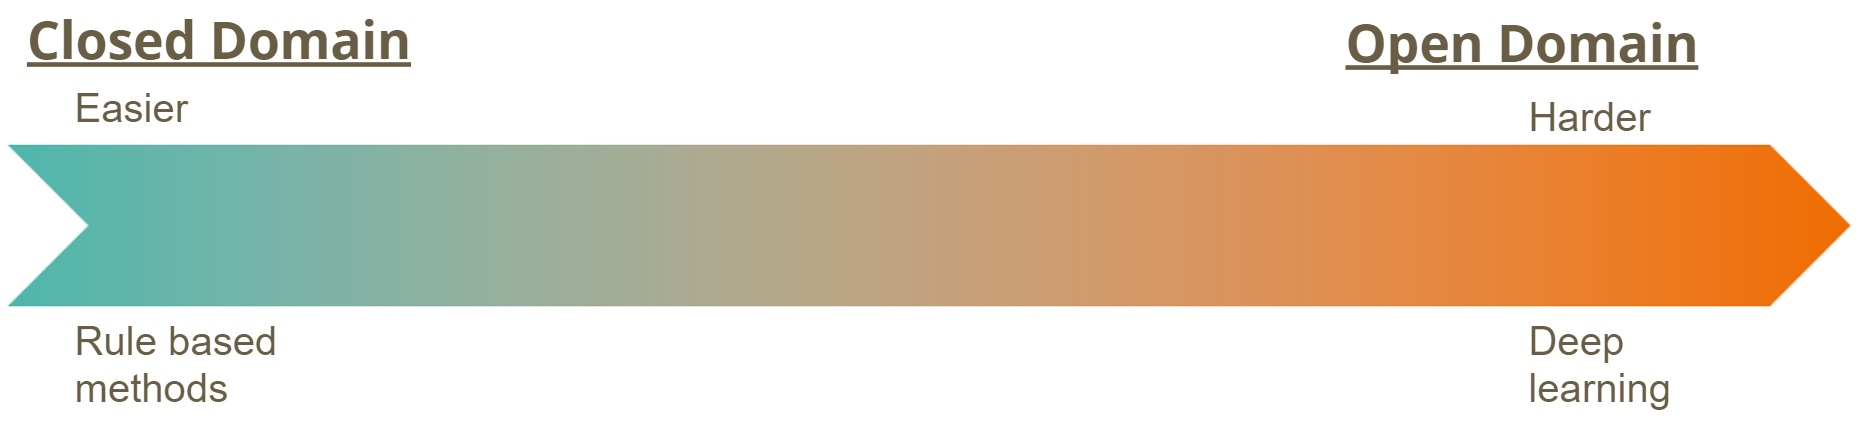
\includegraphics[width=\linewidth]{closedOpenDomainArrow.jpg}
  \caption{Arrow representation of closed vs.open domain}
  \label{fig:closedOpenDomainArrow}
\end{figure}

As \autoref{fig:closedOpenDomainArrow} shows, we have made the observation that for a closed domain the rule based methods work well and the more open the domain is - the harder it gets - the more deep learning is used.

These are no hard borders, as most chatbots fill fall somewhere along this axis (e.g. Helpdesk ). But in general we can say that the task gets more difficult, the more open a domain is. For the closed domain we can easily use rule-based approaches and for open domain deep learning makes more sense. 




\section{State of the art approaches}
In this section we are taking a look at the most commonly used methods to keep track of context in a conversation.
\subsection{Rule-based approaches}
This is the most simple form of keeping track of the context. Most commercial systems use a hand-crafted approach\cite{williams2013dialog}. A fixed set of heuristics decides what to do in which situation. 
The given input is always matched to \textbf{one} specific output state. 

\begin{figure}[H]
\centering
   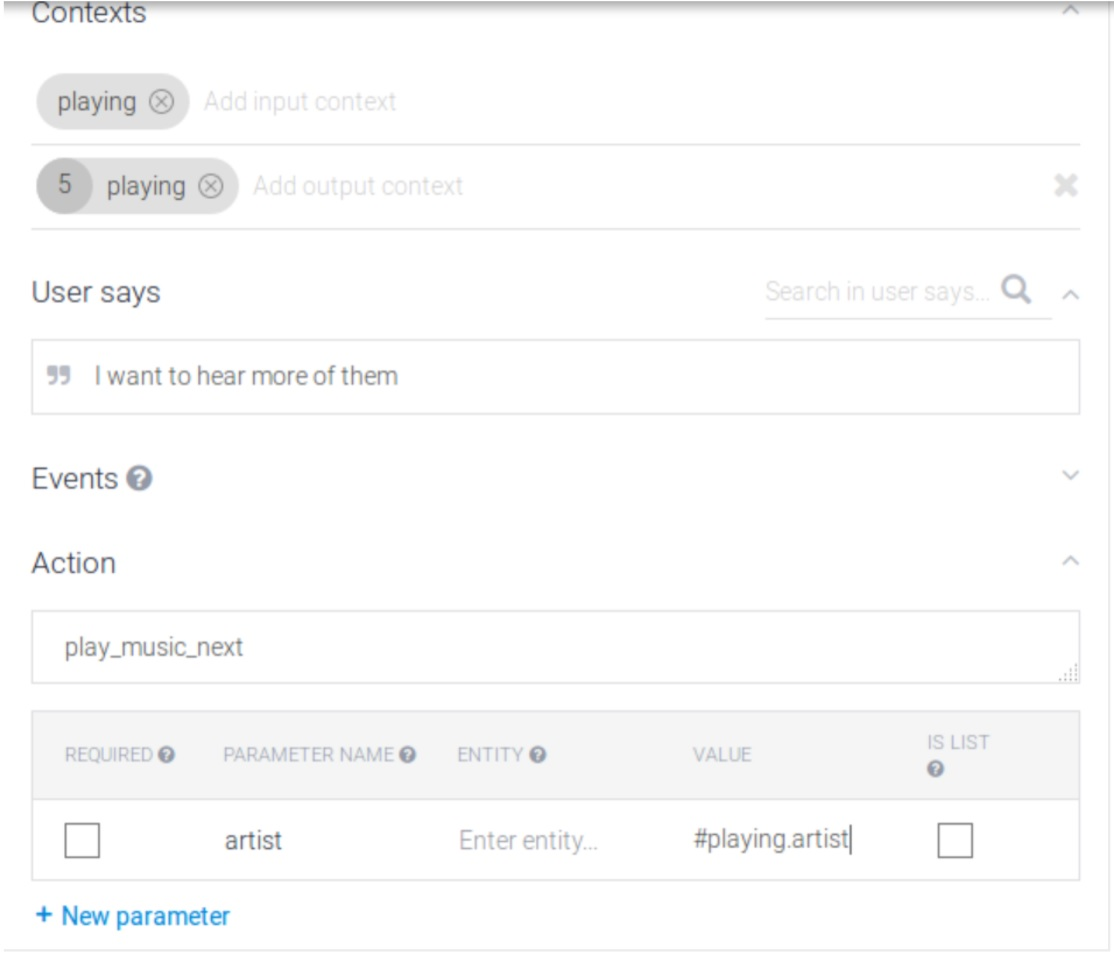
\includegraphics[width=\linewidth]{ruleBasedDialogflow.jpg}
  \caption{Example of a rule-based approach from \url{www.dialogflow.com}}
  \label{fig:dialogFlowExample}
\end{figure}

In \autoref{fig:dialogFlowExample} we can see an example of a rule-based approach. How it works is, that if the user says something similar to "I want to hear more of them", then it recognizes the input context as "playing music" and it will start playing more music of the artist that is currently playing.

Of course this whole process is impossible in an open domain, because the possible set of conversation status is infinitely and we can not create an infinite amount of hand crafted rules to match it and the rules would fail to work for unexpected utterances\cite{wallace2009anatomy}.

\subsection{Probabilistic approaches}
One of the most common and most successful approaches in this field is using a partially observable markov decision process(POMDP)\cite{kaelbling1998planning}\cite{young2013pomdp} dialogue state model. The most successful is the hidden information state (HIS) approach to dialogue management\cite{young2007hidden}\cite{young2010hidden}, which is based on POMDP.

\subsubsection{POMDP}

The partially observable decision process is described by the following:
\begin{itemize}
\item{a set of states $S=\left \{ s_{1},s_{2},....s_{|S|}  \right \}$}
\item{a set of actions $A=\left \{ a_{1},a_{2},....a_{|A|}  \right \}$}
\item{a set of transition probabilities $T(s_{i},a,s_{j})=p(s_{j}|s_{i},a)$}
\item{a set of observation probabilities $O(z_{i},a,s_{j})=p(z_{i}|s_{j},a)$}
\item{a set of rewards $R:S\times A\rightarrow \mathbb{R}$}
\item{a discount factor $\gamma \in \left [ 0,1 \right ]$}
\item{an initial belief $p_{0}(s)$}
\end{itemize}

\begin{figure}[H]
\centering
   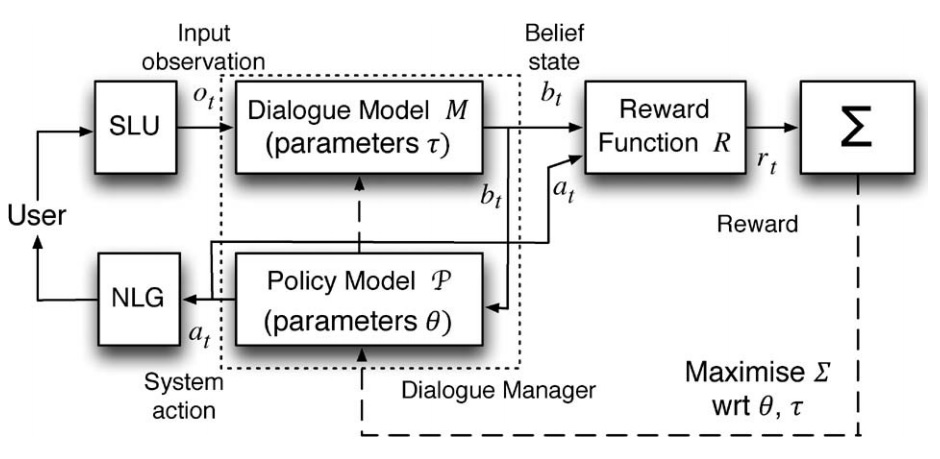
\includegraphics[width=\linewidth]{pomdp.jpg}
  \caption{Partially observable markov decision process (POMDP) based spoken dialogue system.\cite{young2013pomdp} }
  \label{fig:pomdp}
\end{figure}


Because state $s_{t}$ is not observable and thus is not known exactly, a distribution over all possible states is kept. This distribution is called the belief state. So the probability of being in state $s_{t}$, given the belief state \textbf{b} is b($s_{t}$)\cite{young2007hidden}. 
Based on the current belief state \textbf{b} an action $a_{t}$ is selected and the system receives  a reward R and transitions to a new state $s'_{t}$, which is also unobserved. The system then receives an observation o' which depends on $s'_{t}$ and $a_{t}$. After this the belief b is updated\cite{young2007hidden,young2013pomdp}.


The HIS model refines the way the belief monitoring works. A N-best list of beliefs is kept. There is also always a "Rest" value kept in the N-best list (See \autoref{fig:dstChallengeProbabilistic})\cite{young2007hidden}.

\begin{figure}[H]
\centering
   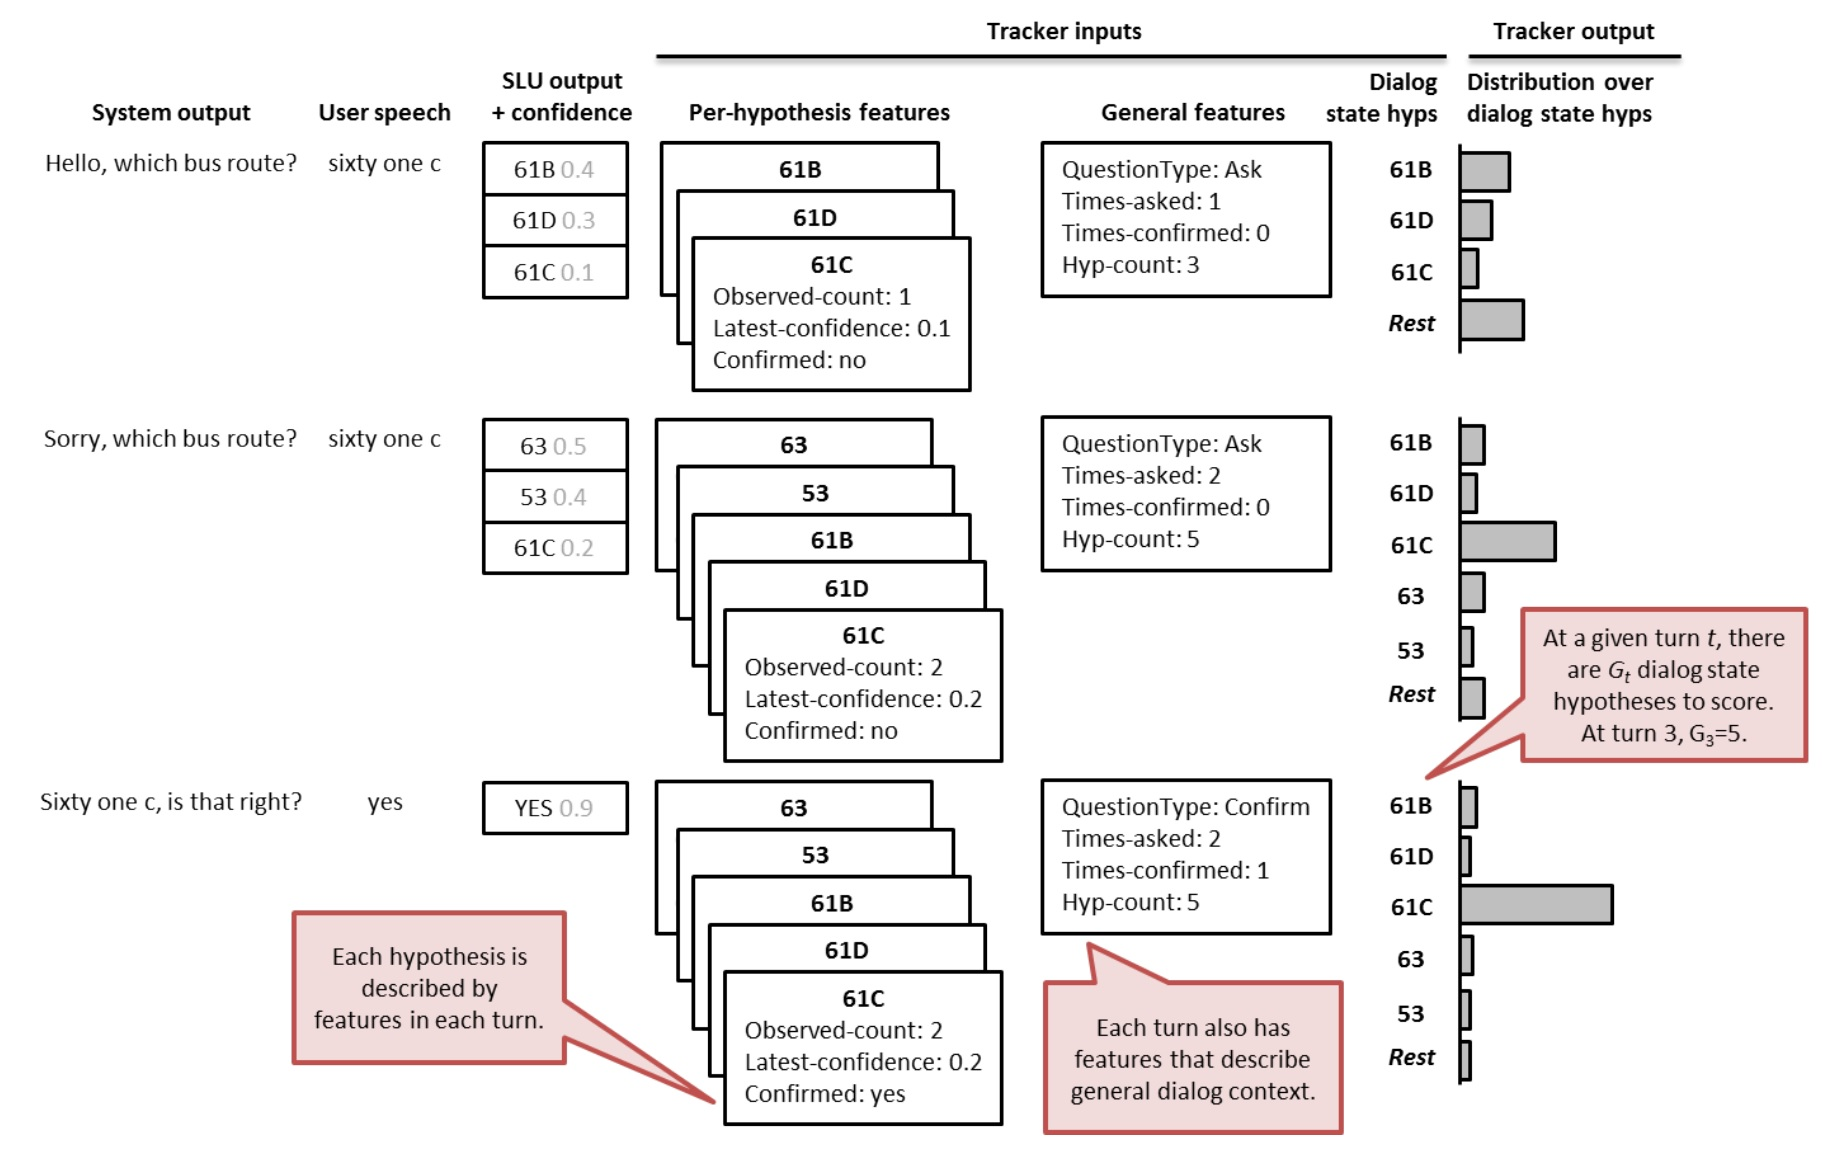
\includegraphics[width=\linewidth]{dstChallangeProbabilistic.jpg}
  \caption{Example of probabilistic dialogue state tracking process\cite{williams2013dialog}.}
  \label{fig:dstChallengeProbabilistic}
\end{figure}

In \autoref{fig:dstChallengeProbabilistic} we can see a nice example of how a probabilistic model works. The example is taken from the dialogue state tracking challenge\cite{williams2013dialog}. We have given a set of states and their possible output hypotheses.
After the user gives the input, the most probable hypothesis is chosen based on the given start probabilities. In the example after the first input, no decision can be made. So the system asks the user for clarification. The probabilities get updated based on the last input and now the correct answer can be given to the user with the updated probabilities. 


\begin{figure}[H]
\centering
   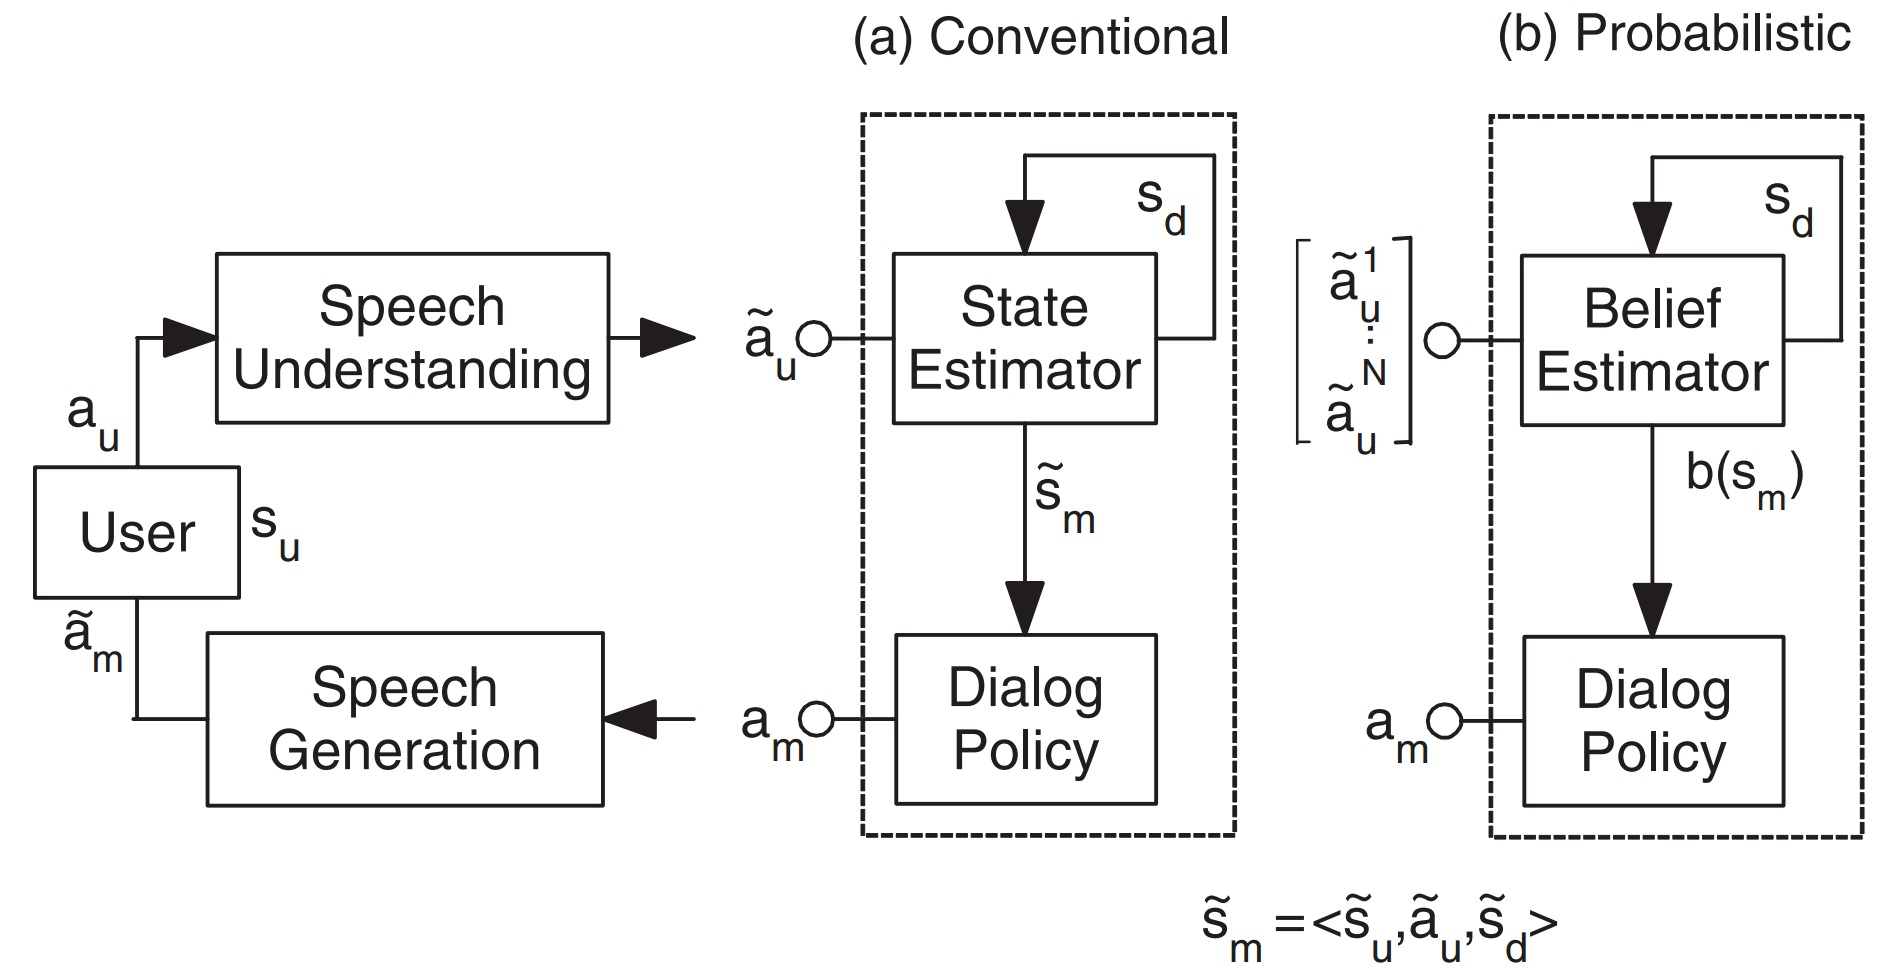
\includegraphics[width=\linewidth]{probabilisticVsConventionalModel.jpg}
  \caption{Conventional model vs. probabilistic POMDP model\cite{young2010hidden}.}
  \label{fig:pomdpVsConventional}
\end{figure}

In \autoref{fig:pomdpVsConventional} we can see two different structures of a spoken dialogue system. In (a) we see a conventional rule-based one and in (b) a probabilistic one. $a_{u}$ and $a_{m}$ denote user and machine dialogue acts, $s_{u}$ is the user goal and $s_{d}$ is the dialogue history. The tilde indicates an estimate.
The conventional dialogue manager in part (a) only holds the estimate of one single state, whereas the probabilistic manager in part (b) represents a dialogue manager which maintains a distribution over all states and accepts an N-best list of alternative user inputs\cite{young2010hidden}.  

\subsection{Data driven approaches}
In a open domain it quickly becomes impossible to define all possible states and state transition. It is therefore not possible to handcraft a system which solves the context state tracking problem\cite{radlinski2017theoretical}.

But with the rise of big data and the large amount of conversations happening on the web, we can use data driven approaches to circumvent this problem. Instead of handcrafting a the mapping from context to response, we can learn this mapping from the data.

In general there are two conrasting data driven approaches; \emph{Discriminative and Generative}.Most produnction systems today use the disctiminative approach, but the research focus is mostly on the generative approach. For both approaches there are statistical and deep learning methods available\cite{yan2016shall}.

\subsubsection{Discriminative methods}
The discriminative approach is to have a (very) large database of predefined responses and then pick the most appropriate one based on the context. This basicly reduces the task to a retreval problem akin to search engines (retreaving results based on a querry).

Most discriminative methods use the data to learn a ranking function. This function is then used to score all possoble responses. The best scoring response is given as an answer to the user.\cite{yan2016shall}

This methods have the advantage that they do not make grammatical or semantical errors (because the predefined responses were weitten by humans). But they can't handle unseen cases or refer back to contextal entities (e.g. names).

An example for a statistical method ist \emph{Okapi BM25}\cite{manning2008introduction}. A search engine ranking function based on "bag-of-words" retreaval.

Is is also possible to train an artificial neural network to score replies\cite{yan2016shall,lowe2015ubuntu}. This method is further explained in section \note{insert section}, as we further investigate this method in our ablation study.

\subsubsection{Generative methods}
Generative methods do not use predefined responses. They generate new responses from scratch. To do this they use approaches from machine translation. But instead of translating form one language to another they translate from context to response.

This has the benefit that it is possible to refer back to enteties in the imput. But these methods often makes grammatical mistakes and are hard to train. They tend to default to "save" answers like "I dont know" or even "I love you".\

There are some methods from statistical machine translation, which basicly try to match the phrase probability distribution in both “languages”. But the research focus lies on deep learning methods like the RNN Encoder-Decoder Networt\cite{sutskever2014sequence}. It uses one network to encode the context into a vector and another to decode the network into the response.

\begin{figure}[H]
\centering
   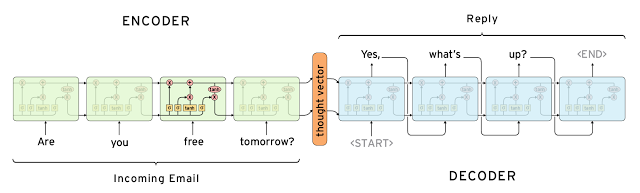
\includegraphics[width=\linewidth]{sequence_to_sequence.png}
  \caption{The dual encoder model form the sequence to sequence paper\cite{sutskever2014sequence}}
  \label{fig:dstChallengeProbabilistic}
\end{figure}

\section{Ablation Study}
\subsection{Goal}
\subsection{Dataset}
\subsection{Model architecture}
\subsection{Methology}
\subsection{Results}





% An example of a floating figure using the graphicx package.
% Note that \label must occur AFTER (or within) \caption.
% For figures, \caption should occur after the \includegraphics.
% Note that IEEEtran v1.7 and later has special internal code that
% is designed to preserve the operation of \label within \caption
% even when the captionsoff option is in effect. However, because
% of issues like this, it may be the safest practice to put all your
% \label just after \caption rather than within \caption{}.
%
% Reminder: the "draftcls" or "draftclsnofoot", not "draft", class
% option should be used if it is desired that the figures are to be
% displayed while in draft mode.
%
%\begin{figure}[!t]
%\centering
%\includegraphics[width=2.5in]{myfigure}
% where an .eps filename suffix will be assumed under latex, 
% and a .pdf suffix will be assumed for pdflatex; or what has been declared
% via \DeclareGraphicsExtensions.
%\caption{Simulation Results}
%\label{fig_sim}
%\end{figure}

% Note that IEEE typically puts floats only at the top, even when this
% results in a large percentage of a column being occupied by floats.


% An example of a double column floating figure using two subfigures.
% (The subfig.sty package must be loaded for this to work.)
% The subfigure \label commands are set within each subfloat command, the
% \label for the overall figure must come after \caption.
% \hfil must be used as a separator to get equal spacing.
% The subfigure.sty package works much the same way, except \subfigure is
% used instead of \subfloat.
%
%\begin{figure*}[!t]
%\centerline{\subfloat[Case I]\includegraphics[width=2.5in]{subfigcase1}%
%\label{fig_first_case}}
%\hfil
%\subfloat[Case II]{\includegraphics[width=2.5in]{subfigcase2}%
%\label{fig_second_case}}}
%\caption{Simulation results}
%\label{fig_sim}
%\end{figure*}
%
% Note that often IEEE papers with subfigures do not employ subfigure
% captions (using the optional argument to \subfloat), but instead will
% reference/describe all of them (a), (b), etc., within the main caption.


% An example of a floating table. Note that, for IEEE style tables, the 
% \caption command should come BEFORE the table. Table text will default to
% \footnotesize as IEEE normally uses this smaller font for tables.
% The \label must come after \caption as always.
%
%\begin{table}[!t]
%% increase table row spacing, adjust to taste
%\renewcommand{\arraystretch}{1.3}
% if using array.sty, it might be a good idea to tweak the value of
% \extrarowheight as needed to properly center the text within the cells
%\caption{An Example of a Table}
%\label{table_example}
%\centering
%% Some packages, such as MDW tools, offer better commands for making tables
%% than the plain LaTeX2e tabular which is used here.
%\begin{tabular}{|c||c|}
%\hline
%One & Two\\
%\hline
%Three & Four\\
%\hline
%\end{tabular}
%\end{table}


% Note that IEEE does not put floats in the very first column - or typically
% anywhere on the first page for that matter. Also, in-text middle ("here")
% positioning is not used. Most IEEE journals/conferences use top floats
% exclusively. Note that, LaTeX2e, unlike IEEE journals/conferences, places
% footnotes above bottom floats. This can be corrected via the \fnbelowfloat
% command of the stfloats package.



\section{Conclusion}
The conclusion goes here.\cite{chopra2017my}




% conference papers do not normally have an appendix


% use section* for acknowledgement





% trigger a \newpage just before the given reference
% number - used to balance the columns on the last page
% adjust value as needed - may need to be readjusted if
% the document is modified later
%\IEEEtriggeratref{8}
% The "triggered" command can be changed if desired:
%\IEEEtriggercmd{\enlargethispage{-5in}}

% references section

% can use a bibliography generated by BibTeX as a .bbl file
% BibTeX documentation can be easily obtained at:
% http://www.ctan.org/tex-archive/biblio/bibtex/contrib/doc/
% The IEEEtran BibTeX style support page is at:
% http://www.michaelshell.org/tex/ieeetran/bibtex/
\bibliographystyle{IEEEtran}
% argument is your BibTeX string definitions and bibliography database(s)
\bibliography{IEEEabrv,bibliography}
%
% <OR> manually copy in the resultant .bbl file
% set second argument of \begin to the number of references
% (used to reserve space for the reference number labels box)
%\begin{thebibliography}{1}

%\bibitem{IEEEhowto:kopka}
%H.~Kopka and P.~W. Daly, \emph{A Guide to \LaTeX}, 3rd~ed.\hskip 1em plus
%  0.5em minus 0.4em\relax Harlow, England: Addison-Wesley, 1999.

%\end{thebibliography}




% that's all folks
\end{document}


